\section{Code structure} 
NB : All the code is given in the section \ref{Code}.

\begin{itemize}
    \item[$\bullet$] \textbf{Variables:}
    \begin{itemize}
        \item[-] \texttt{BALL\_X} : the horizontal position of the ball, which can take values between 0 and 6\\
        
        \item[-] \texttt{BALL\_Y}  : the vertical position of the ball, which can take values between 0 and 4\\
        
        \item[-] \texttt{PADDLE\_X} : the horizontal position of the left corner of the paddle, which can take values between 0 and 5\\
        
        \item[-] \texttt{RAND\_X} : a number generated to randomly determine the position of the ball when it hits the top wall\\
        
        \item[-] \texttt{BALL\_DIRECTION} : direction of the ball's movement, can be \textit{up} or \textit{down}\\
        
        \item[-] \texttt{GAME\_STATE} : indicates the state of the game, it can be $game\_start$ (before the start of a game), $game\_play$ (when a game is in progress) or $game\_over$ (when you have lost) \\
        
        \item[-] \texttt{LIVES} : are decremented when the ball hits the bottom wall, take values from 3 to 0
        
        \begin{figure}[H]
        \centering
        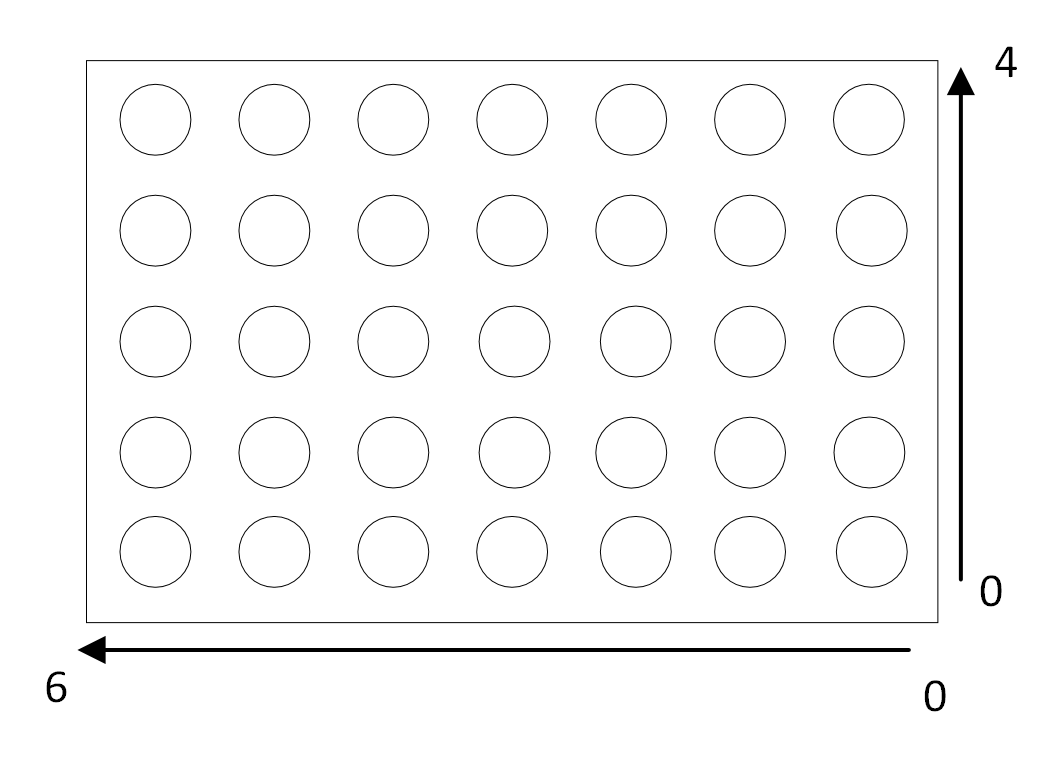
\includegraphics[scale = 0.25]{Ressources/png/Dessin1.png}
        \caption{Visualization of the coordinates chosen for the LED matrix}
\end{figure}
        
    \end{itemize}
    \item[$\bullet$] \textbf{Processes:} 
    \begin{itemize}
        \item[-] \textit{Random} : generates a number to randomly determine the position of the ball when it hits the top wall. It is triggered at the rising edge of the \texttt{CLK\_FAST}. It goes from 0 to 6 and when it's value is equal to 6, it returns to 0. The computation of the next value of our ball position on the top wall is only done triggering the \texttt{CLK\_SLOW} which assure that our number is random.\\
        
        \item[-] \textit{paddle movement} : if one of the button (left or right) is pressed, we check if the paddle can go in the desired direction. If so, the paddle moves in the direction wanted. It is triggered by the \texttt{CLK\_SLOW}.\\
        
        \item[-] \textit{ball movement} : Triggered by the \texttt{CLK\_SLOW}, this process handles the movement of the ball and the collisions with the paddle. There are 4 types of collisions in this implementation : 
        \begin{itemize}
            \item[-] paddle collision : if the ball is at the bottom wall, we check if its horizontal position corresponds to one of the two points of the paddle. If it collides, the ball will go up by changing \texttt{BALL\_DIRECTION} to \textit{up}\\
            
            \item[-] bottom collision : if the ball is at the bottom wall but there is not a collision with the paddle, \texttt{LIVES} is decremented and the ball will start at a random position at the top wall\\

            \item[-] top collision : when the ball is at the top, its position is updated with random position x and the ball will start going down from that new position \\

            \item[-] no collision : handles the cases when the ball is between the top and the bottom wall. It checks the \texttt{BALL\_DIRECTION} and increments \texttt{BALL\_Y} if it is \textit{up} or decrements it if it is \textit{down}
        \end{itemize}
        
        \hangindent=\labelwidth \hangafter=0 When the reset button is pressed, this process is responsible of giving a new random \hangindent=\labelwidth \hangafter=0 horizontal position at the top row.
        
        \item[-] \textit{display} : Before the game starts, '\textbf{P}' is shown on the LED matrix. When the game is playing, it displays the correct LEDs and when the game is over, it displays a cross on the matrix. It is triggered by the \texttt{CLK\_FAST} to have the correct fluency for the LEDs.\\

        \item[-] \textit{state management} : manages the states of the games. When the start button is pressed, it starts the game by putting \texttt{GAME\_STATE} at $game\_play$. The game goes on until there are no more lives remaining. Once the game is done,  \texttt{GAME\_STATE} is set at $game\_over$. 
    \end{itemize}
\end{itemize}
